\chapter{Tráfego de membranas e endereçamento de proteínas}\label{ch:b3:membrane-traffic}

Uma célula do pâncreas produz uns dez milhões de moléculas de enzima
digestiva por minuto, empacota-as em grânulos e as libera num ducto a
um sinal vindo do intestino --- sem jamais deixar solta uma molécula de
tripsina no próprio citoplasma. Uma célula do fígado retira colesterol
do sangue engolindo inteiras as partículas que o carregam, a uma taxa
de milhares por minuto, e devolve cada receptor à superfície para a
próxima. Uma proteína recém-feita destinada à mitocôndria, ao núcleo,
ao \omterm{def:b3:membrane-traffic:endocytosis}{lisossomo}, à membrana ou ao mundo exterior chega a seu endereço
entre uma dúzia de compartimentos com uma taxa de erro que
envergonharia um serviço postal. Este capítulo trata do endereçamento:
os sinais escritos nas proteínas, as máquinas que os leem, as vesículas
que levam membrana e carga entre compartimentos, os \omterm{def:b3:membrane-traffic:coats}{revestimentos} que
moldam as vesículas e as proteínas que as fazem fundir-se com o alvo
certo, e o tráfego de mão dupla --- secreção para fora, endocitose para
dentro --- que uma célula eucarionte mantém a cada segundo de sua vida.

\section{Sinais e endereços}

\begin{definition}[Sinais de endereçamento]\label{def:b3:membrane-traffic:signals}
\index{sinal de endereçamento}\index{peptídeo-sinal}\index{sinal de localização nuclear}\index{pré-sequência}
Um \emph{sinal de endereçamento} é um segmento de uma proteína, ou uma
modificação dela, lido por um receptor que entrega a proteína a um
compartimento. O \emph{peptídeo-sinal}, um trecho de
\numrange{15}{30} resíduos na extremidade amino com um cerne
hidrofóbico, manda a proteína para o retículo endoplasmático enquanto
ela está sendo feita; dali a rota padrão leva pelo Golgi até a membrana
plasmática ou o exterior, e sinais adicionais desviam para o \omterm{def:b3:membrane-traffic:endocytosis}{lisossomo}
(um açúcar fosforilado) ou de volta ao retículo (a sequência
carboxi-terminal KDEL). Um \emph{sinal de localização nuclear}, um
curto trecho básico como PKKKRKV, é ligado por importinas que levam a
proteína enovelada pelo poro nuclear; uma \emph{pré-sequência}
mitocondrial, uma hélice anfipática de \numrange{20}{50} resíduos, é
reconhecida por receptores da membrana externa e enfiada, desenovelada,
pelas translocases das duas membranas; as enzimas peroxissomais
terminam em SKL. As proteínas sem nenhum desses sinais ficam no
citosol. Todo sinal foi descoberto do mesmo modo: deletá-lo deixa a
proteína no citosol, enxertá-lo numa proteína citosólica manda essa
proteína ao compartimento.
\end{definition}

\begin{proof}[Evidência]
Blobel e Dobberstein (1975) traduziram o RNA mensageiro de uma cadeia
leve de anticorpo num sistema livre de células. Sem membranas o produto
era cerca de vinte resíduos mais longo que a proteína secretada; com
fragmentos de retículo endoplasmático acrescentados \emph{durante} a
tradução, o produto tinha o tamanho da secretada e ficava protegido da
protease acrescentada --- estava dentro das vesículas ---, ao passo que
membranas acrescentadas depois da tradução não faziam nada. O segmento
amino-terminal extra, o \omterm{def:b3:membrane-traffic:signals}{peptídeo-sinal}, é necessário para entrar no
retículo, é removido dentro dele e só funciona enquanto a cadeia está
sendo feita: a \emph{hipótese do sinal}, confirmada em cada detalhe
quando o receptor (a partícula de reconhecimento do sinal, Walter e
Blobel, 1981) e o canal (Sec61) foram purificados.
\end{proof}

\begin{omfigure}
\begin{tikzpicture}[every node/.style={font=\scriptsize}, >=stealth]
  % ER membrane
  \fill[omDef!15] (0,0) rectangle (12,-1.6);
  \draw[very thick, omDef] (0,0) -- (12,0); \draw[very thick, omDef] (0,-0.35) -- (12,-0.35);
  \node[right, omDef!70!black] at (0.1,-1.3) {lúmen do RE};
  \node[right] at (0.1,2.9) {citosol};
  % stage 1: ribosome with emerging signal peptide + SRP
  \draw[thick, fill=gray!25] (1.4,1.6) circle (0.5); \draw[thick, fill=gray!25] (1.4,0.95) ellipse (0.62 and 0.3);
  \draw[very thick, omThm] (1.4,0.65) -- (1.4,0.2) -- (1.9,0.1);
  \draw[thick, fill=omProp!40] (2.1,0.35) ellipse (0.35 and 0.2); \node[above right] at (2.2,0.5) {SRP};
  \node[below, align=center] at (1.7,-1.7) {1. o peptídeo-sinal emerge;\\a SRP se liga, a tradução pausa};
  % stage 2: docking at SRP receptor and translocon
  \draw[->, thick] (3.2,1.2) -- (4.2,1.2);
  \draw[thick, fill=gray!25] (5.6,1.75) circle (0.5); \draw[thick, fill=gray!25] (5.6,1.1) ellipse (0.62 and 0.3);
  \draw[thick, fill=omMeth!40] (5.2,0.0) rectangle (5.45,-0.35); \draw[thick, fill=omMeth!40] (5.75,0.0) rectangle (6.0,-0.35);
  \node[below, align=center] at (5.9,-1.7) {2. o receptor de SRP o acopla\\ao Sec61; a SRP sai};
  \draw[very thick, omThm] (5.6,0.8) -- (5.6,-0.2);
  \draw[thick, fill=omProp!40] (4.7,0.15) ellipse (0.3 and 0.18); \node[above] at (4.7,0.33) {receptor de SRP};
  % stage 3: translocation, cleavage, glycosylation
  \draw[->, thick] (7.2,1.2) -- (8.2,1.2);
  \draw[thick, fill=gray!25] (9.6,1.75) circle (0.5); \draw[thick, fill=gray!25] (9.6,1.1) ellipse (0.62 and 0.3);
  \draw[thick, fill=omMeth!40] (9.2,0.0) rectangle (9.45,-0.35); \draw[thick, fill=omMeth!40] (9.75,0.0) rectangle (10.0,-0.35);
  \draw[very thick, omThm] (9.6,0.8) -- (9.6,-0.5) .. controls (9.6,-1.0) and (10.3,-1.1) .. (10.6,-0.7);
  \draw[omThm, thick] (10.9,-0.9) -- (11.2,-0.9); \node[right, font=\tiny] at (11.0,-1.15) {sinal cortado};
  \fill[omExo] (10.3,-1.0) circle (0.07); \fill[omExo] (10.45,-1.12) circle (0.07); \node[below, font=\tiny] at (10.2,-1.15) {açúcares};
  \node[below, align=center] at (10.0,-1.7) {3. a cadeia atravessa enquanto é feita;\\sinal cortado, açúcares acrescentados};
\end{tikzpicture}

{\small A hipótese do sinal. Um \omterm{def:b3:membrane-traffic:signals}{peptídeo-sinal} no início da cadeia
nascente é ligado pela partícula de reconhecimento do sinal, que pausa
a tradução e acopla o ribossomo ao canal Sec61; a cadeia então
atravessa a membrana à medida que é sintetizada, o sinal é cortado no
lúmen e açúcares são acrescentados.}
\end{omfigure}

\begin{proposition}[Proteínas de membrana e topologia]\label{prop:b3:membrane-traffic:topology}
\index{sequência de parada de transferência}\index{topologia de membrana}
Um trecho hidrofóbico de cerca de vinte resíduos no meio de uma cadeia
em translocação age como \emph{\omterm{prop:b3:membrane-traffic:topology}{sequência de parada de transferência}}: o
canal se abre lateralmente e a libera na bicamada como hélice
transmembrana, com a parte já translocada no lúmen e o resto feito para
dentro do citosol. Um segundo trecho desses reinicia a translocação, e
uma proteína com $n$ sinais alternados termina com $n$ hélices que
atravessam a membrana. A orientação fixada no retículo nunca muda: o
que dá para o lúmen do retículo dá para o lúmen do Golgi e de cada
vesícula depois dele, e para o \emph{exterior} da célula depois da
fusão com a membrana plasmática. Daí que os açúcares, acrescentados
apenas no lúmen, estejam sempre na face extracelular de uma proteína de
superfície, e que a topologia de um receptor possa ser lida a partir de
onde estão seus sítios de glicosilação.
\end{proposition}

\begin{method}[Pulso--caça]\label{met:b3:membrane-traffic:pulse-chase}
\index{pulso--caça}\index{autorradiografia}
Para acompanhar uma população de moléculas recém-feitas pela célula:
(1) exponha as células brevemente (o \emph{pulso}, alguns minutos) a um
precursor radioativo ou marcado de outro modo --- leucina tritiada para
proteínas; (2) substitua-o por um excesso de precursor não marcado (a
\emph{caça}), de modo que nenhuma marcação nova seja incorporada; (3)
fixe amostras de células em intervalos e localize a marcação por
autorradiografia em micrografias eletrônicas, ou isolando os
compartimentos e contando; (4) represente a fração de marcação em cada
compartimento contra o tempo. A ordem em que os compartimentos enchem e
esvaziam é a rota; os tempos dão o tempo de residência em cada um. O
laboratório de Palade (anos 1960) aplicou o método à célula acinar
pancreática e encontrou a marcação no retículo rugoso aos \qty{3}{min},
no Golgi aos \qty{20}{min}, em vacúolos de condensação e grânulos aos
\qty{40}{min}, e no ducto depois de uma hora e de um sinal: a via
secretora, disposta no tempo.
\end{method}

\begin{theorem}[Compartimentos em sequência e as curvas de pulso--caça]\label{thm:b3:membrane-traffic:pulse-chase}
\index{modelo de compartimentos}
Seja um pulso de proteína marcada que deixa o compartimento $A$ rumo a
$B$ com taxa de primeira ordem $k_{1}$ e deixa $B$ rumo a $C$ com taxa
$k_{2}$, retendo-a $C$. Com toda a marcação em $A$ em $t = 0$,
\[
A(t) = e^{-k_{1}t},\qquad
B(t) = \frac{k_{1}}{k_{2} - k_{1}}\bigl(e^{-k_{1}t} - e^{-k_{2}t}\bigr),
\qquad
C(t) = 1 - A - B,
\]
e a marcação em $B$ tem um pico em
$t^{*} = \ln(k_{2}/k_{1})/(k_{2} - k_{1})$. O tempo médio de residência
em $A$ é $1/k_{1}$ e em $B$ é $1/k_{2}$, seja qual for a ordem das duas
taxas.
\end{theorem}
\begin{proof}
$\mathrm{d}A/\mathrm{d}t = -k_{1}A$ dá a exponencial. Para $B$,
$\mathrm{d}B/\mathrm{d}t = k_{1}A - k_{2}B = k_{1}e^{-k_{1}t} - k_{2}B$;
tente $B = \beta(e^{-k_{1}t} - e^{-k_{2}t})$: a derivada é
$\beta(-k_{1}e^{-k_{1}t} + k_{2}e^{-k_{2}t})$ e $-k_{2}B = \beta(-k_{2}
e^{-k_{1}t} + k_{2}e^{-k_{2}t})$, de modo que a equação exige $\beta(k_{2}
- k_{1})e^{-k_{1}t} = k_{1}e^{-k_{1}t}$, $\beta = k_{1}/(k_{2} -
k_{1})$, e $B(0) = 0$ como se pedia. Fazendo
$\mathrm{d}B/\mathrm{d}t =
0$: $k_{1}e^{-k_{1}t} = k_{2}e^{-k_{2}t}$,
de onde vem $t^{*}$. O tempo médio que uma molécula passa num
compartimento do qual sai à taxa $k$ é $\int_{0}^{
\infty} t\,k e^{-kt}\,\mathrm{d}t = 1/k$.
\end{proof}

\begin{example}[A célula de Palade em números]\label{ex:b3:membrane-traffic:palade}
Tome $k_{1} = \qty{0.1}{min^{-1}}$ (dez minutos no retículo) e
$k_{2} = \qty{0.05}{min^{-1}}$ (vinte no Golgi). O Golgi tem seu pico
em $t^{*} = \ln 2/0.05 = \qty{13.9}{min}$, e contém então
$B = 2(e^{-1.39} -
e^{-0.69}) = 2(0.25 - 0.50)\cdot(-1) = 0.50$: metade
da marcação. Aos \qty{40}{min}, $A = 0.018$,
$B = 2(0.018 - 0.135) \to 0.23$, $C = 0.75$: três quartos da proteína
chegaram aos grânulos. As curvas observadas no laboratório de Palade
têm essa forma, e ajustá-las foi como os tempos de residência foram
medidos pela primeira vez.
\end{example}

\begin{omfigure}
\begin{tikzpicture}
\begin{axis}[
  width=0.7\linewidth, height=5.6cm,
  axis x line=bottom, axis y line=left,
  xmin=0, xmax=80, ymin=0, ymax=1.05,
  xlabel={minutos após o pulso}, ylabel={fração da marcação},
  xlabel style={font=\small, at={(axis description cs:0.5,-0.12)}, anchor=north},
  ylabel style={font=\small},
  tick label style={font=\small}, xtick={0,20,40,60,80}, ytick={0,0.5,1},
  clip=false,
]
\addplot[very thick, omDef, domain=0:80, samples=80] {exp(-0.1*x)};
\addplot[very thick, omProp, domain=0:80, samples=80] {2*(exp(-0.05*x)-exp(-0.1*x))};
\addplot[very thick, omMeth!70!black, domain=0:80, samples=80] {1-exp(-0.1*x)-2*(exp(-0.05*x)-exp(-0.1*x))};
\node[font=\scriptsize, omDef, anchor=south west] at (axis cs:4,0.62) {retículo, $A$};
\node[font=\scriptsize, omProp, anchor=south] at (axis cs:14,0.53) {Golgi, $B$};
\node[font=\scriptsize, omMeth!70!black, anchor=north west] at (axis cs:45,0.72) {grânulos, $C$};
\end{axis}
\end{tikzpicture}

{\small Curvas de pulso--caça do modelo de duas taxas com
$k_{1} =
\qty{0.1}{min^{-1}}$ e $k_{2} = \qty{0.05}{min^{-1}}$: a
marcação deixa o retículo exponencialmente, passa pelo Golgi com um
pico aos \qty{14}{min} e se acumula nos grânulos.}
\end{omfigure}

\section{O retículo endoplasmático: enovelamento, açúcares e qualidade}

\begin{definition}[N-glicosilação e controle de qualidade]\label{def:b3:membrane-traffic:glycosylation}
\index{N-glicosilação}\index{ciclo da calnexina}\index{degradação associada ao RE}\index{resposta a proteínas mal enoveladas}
Quando a cadeia entra no lúmen, um oligossacarídeo pré-montado de
catorze açúcares (duas N-acetilglicosaminas, nove manoses, três
glicoses) é transferido de um carreador lipídico para asparaginas na
sequência Asn-X-Ser/Thr --- a \emph{N-glicosilação}. As três glicoses
são então aparadas uma a uma, e a aparagem é um relógio do
\omterm{def:b3:structural-biology:levels}{enovelamento}: uma proteína que ainda carrega uma glicose é retida pela
\omterm{def:b3:structural-biology:chaperones}{chaperona} calnexina; uma proteína cuja última glicose foi removida mas
que ainda não está enovelada é reglicosilada por uma enzima que
reconhece trechos hidrofóbicos expostos, e volta à calnexina --- o
\emph{ciclo da calnexina}. As proteínas que falham repetidamente são
puxadas de volta ao citosol, ubiquitinadas e destruídas pelo
proteassomo: a \emph{degradação associada ao RE} (ERAD). Quando as
proteínas mal enoveladas se acumulam mais depressa do que podem ser
enoveladas ou destruídas, sensores da membrana do retículo disparam a
\emph{resposta a proteínas mal enoveladas}: a tradução é retardada, os
genes de \omterm{def:b3:structural-biology:chaperones}{chaperonas} são induzidos, o retículo é expandido e, se o
estresse persistir, a célula é morta. A mutação mais comum da fibrose
cística ($\Delta$F508 no CFTR) produz um canal que funcionaria, mas se
enovela devagar demais, é capturado pela ERAD e nunca chega à
superfície; fármacos que o ajudam a enovelar-se são hoje um tratamento.
\end{definition}

\begin{omfigure}
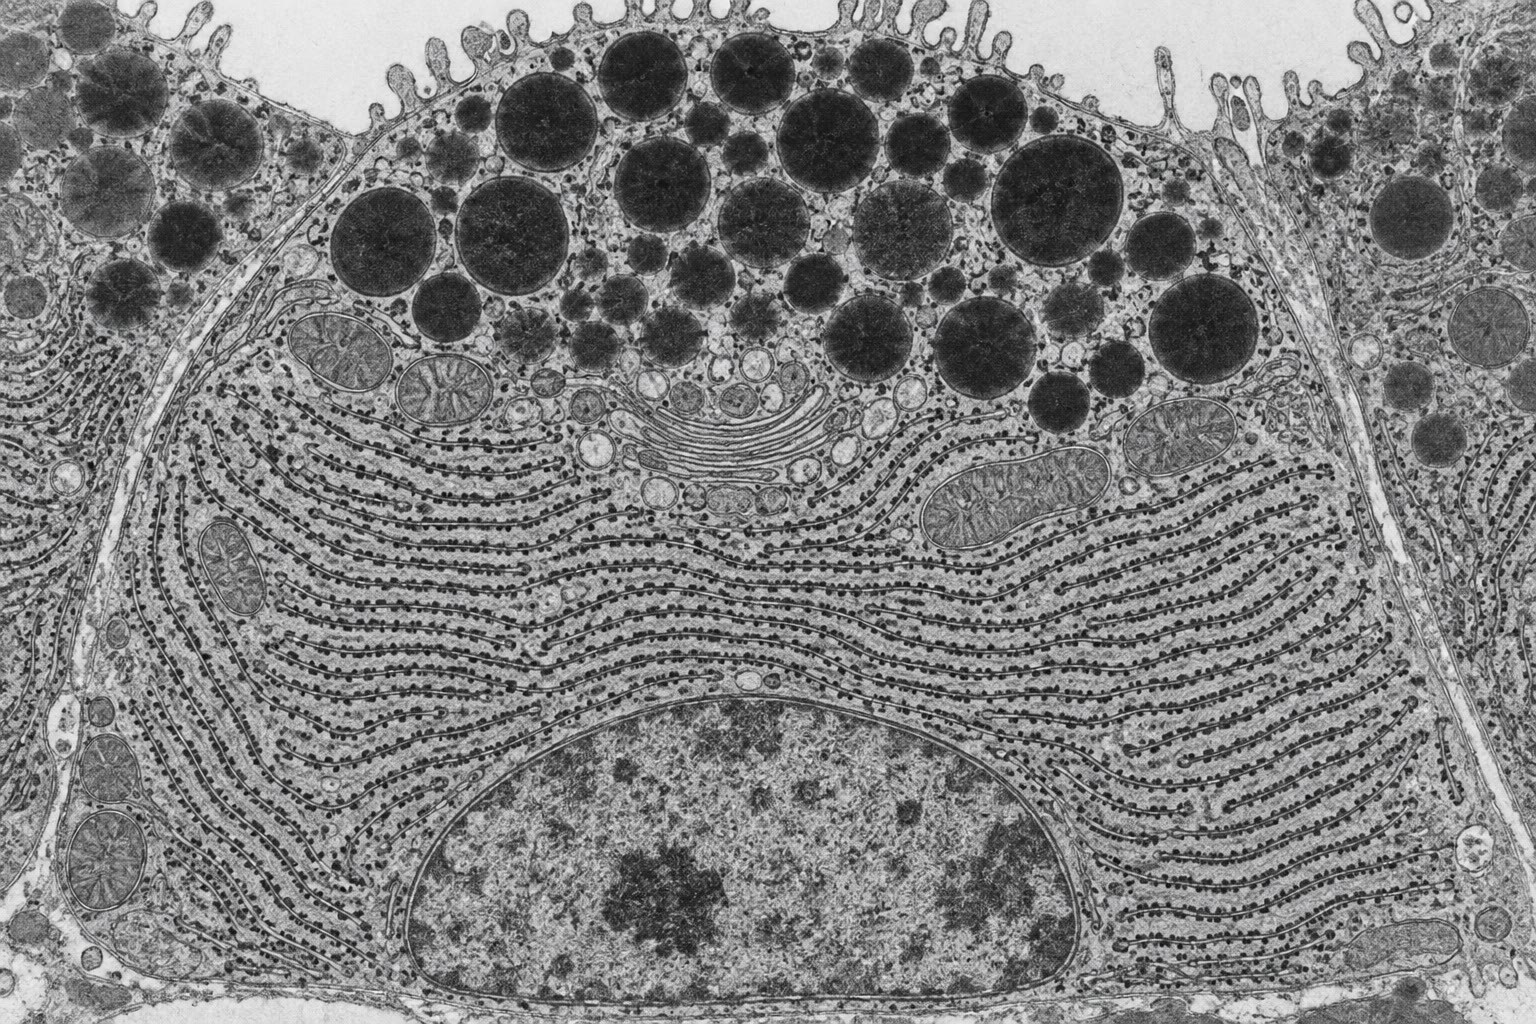
\includegraphics[width=0.56\linewidth]{images/book5/ai/b5-08-pancreas-acinar.jpg}

{\small Uma célula acinar pancreática no microscópio eletrônico:
retículo endoplasmático rugoso empilhado e cravejado de ribossomos
preenche a base, o Golgi fica acima do núcleo, e grânulos secretores
densos de enzima digestiva estão apinhados sob a superfície apical, à
espera de um sinal.}
\end{omfigure}

\section{Vesículas: brotamento, endereçamento, fusão}

\begin{definition}[Revestimentos e brotamento de vesículas]\label{def:b3:membrane-traffic:coats}
\index{vesícula revestida}\index{COPII}\index{COPI}\index{clatrina}\index{GTPase pequena}
Uma vesícula de transporte é moldada por um \emph{revestimento} de
proteínas montado na face citosólica de uma membrana, que curva a
membrana num broto de \qtyrange{60}{100}{nm}, recolhe carga por meio de
receptores que atravessam a membrana e é descartado depois que a
vesícula se destaca. Três revestimentos servem às rotas principais: o
\emph{COPII} para as vesículas que deixam o retículo rumo ao Golgi, o
\emph{COPI} para o tráfego de volta do Golgi ao retículo e entre as
cisternas do Golgi, e a \emph{clatrina} --- uma proteína de três pernas
que polimeriza numa gaiola de hexágonos e pentágonos --- para as
vesículas que deixam o Golgi trans rumo aos \omterm{def:b3:membrane-traffic:endocytosis}{endossomos} e para a
endocitose na membrana plasmática, onde proteínas adaptadoras ligam a
gaiola aos receptores que estão sendo internalizados. Cada revestimento
é recrutado por uma \emph{GTPase pequena} (Sar1 para o COPII, Arf1 para
o COPI e a clatrina) que se insere na membrana em sua forma ligada a
GTP e, ao hidrolisar o GTP depois do brotamento, deixa o revestimento
cair. Sinais de recuperação mantêm os compartimentos distintos: as
proteínas do retículo que escapam carregando KDEL são ligadas no Golgi
por um receptor e levadas de volta em vesículas COPI.
\end{definition}

\begin{omfigure}
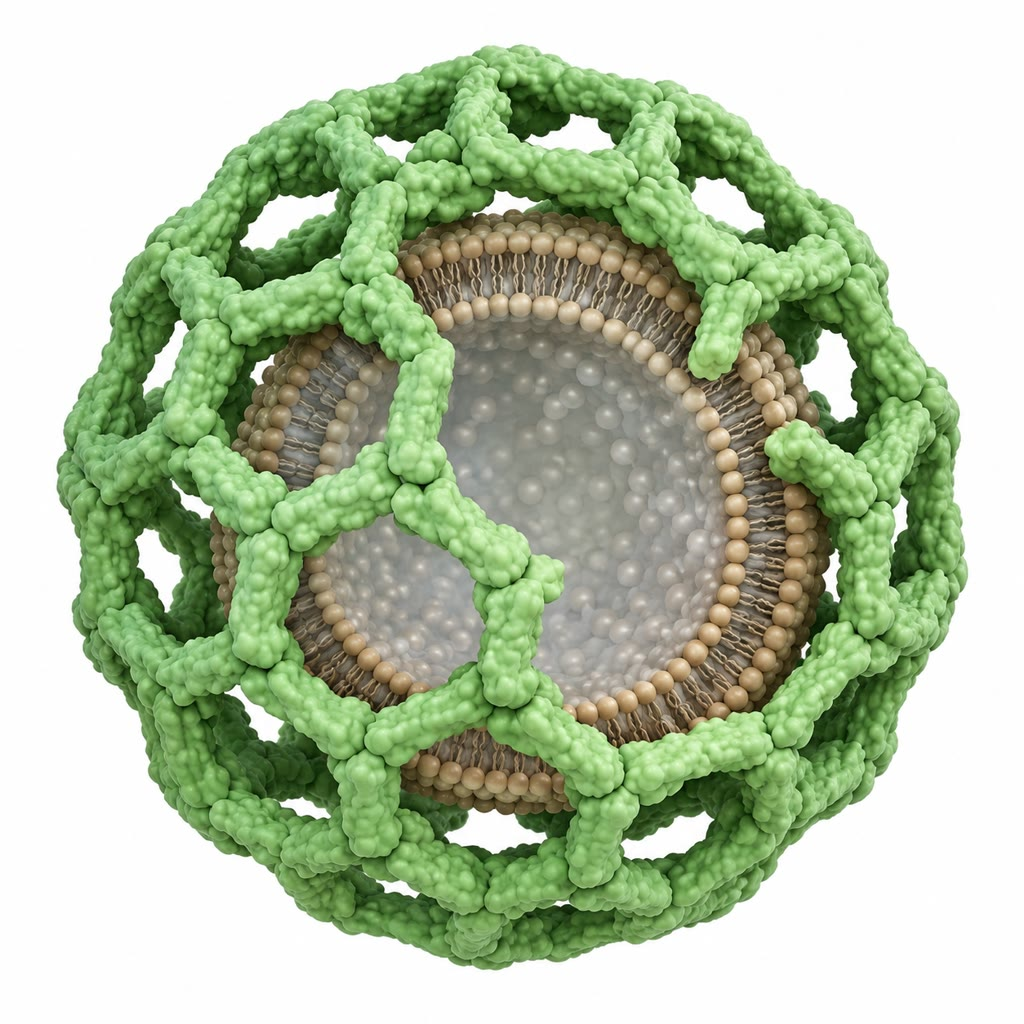
\includegraphics[width=0.36\linewidth]{images/book5/ai/b5-08-clathrin-cage.jpg}\hspace{0.04\linewidth}
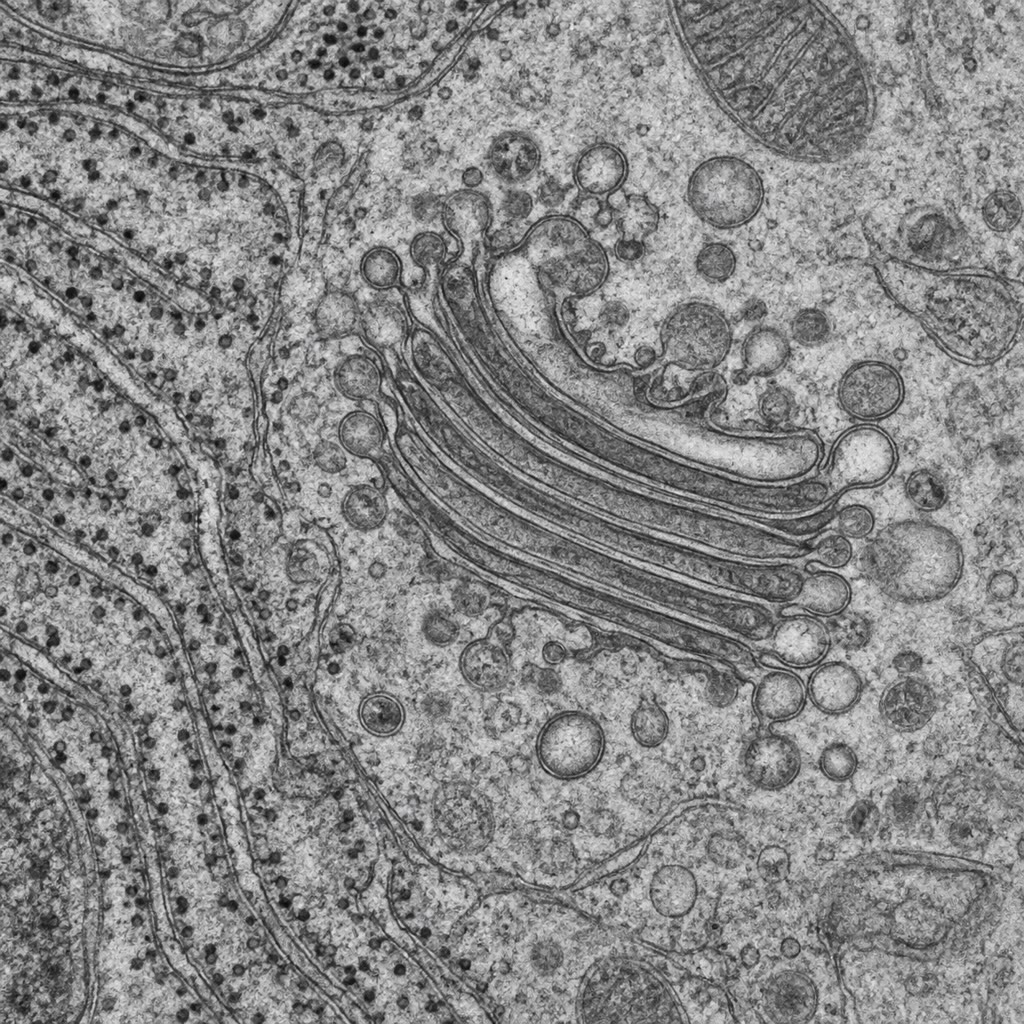
\includegraphics[width=0.36\linewidth]{images/book5/ai/b5-08-golgi-tem.jpg}

{\small À esquerda: uma gaiola de \omterm{def:b3:membrane-traffic:coats}{clatrina}, a rede poliédrica de
unidades de três pernas que molda uma vesícula endocítica (cortada para
mostrar a membrana por dentro). À direita: uma pilha de Golgi no
microscópio eletrônico, um monte de cisternas achatadas com vesículas
brotando das bordas.}
\end{omfigure}

\begin{definition}[Endereçamento e fusão]\label{def:b3:membrane-traffic:fusion}
\index{GTPase Rab}\index{SNARE}\index{fusão de membranas}\index{sinaptotagmina}
Uma vesícula encontra seu alvo por duas camadas de reconhecimento. As
\emph{GTPases Rab} --- umas sessenta numa célula humana, cada uma nas
membranas de um compartimento --- recrutam longas proteínas de amarra
que capturam uma vesícula que chegue carregando a Rab correspondente.
Depois agem as \emph{SNAREs}: uma v-SNARE na vesícula e t-SNAREs no
alvo, proteínas helicoidais ancoradas em suas membranas, enrolam-se uma
na outra das extremidades distais em direção às membranas, e a energia
do feixe de quatro hélices que formam puxa as duas bicamadas até que se
fundam. Cada pareamento de SNAREs é específico, uma segunda conferência
do endereço. Depois da fusão o feixe é desmontado pela ATPase NSF para
reúso. A fusão pode ser feita esperar por um sinal: no terminal nervoso
as SNAREs são mantidas meio fechadas pela complexina até que a
\emph{sinaptotagmina}, ligando o cálcio que entra quando chega um
potencial de ação, complete o fechamento em menos de um milissegundo
--- a liberação de neurotransmissor tratada no volume do 2.º ano. As
neurotoxinas do tétano e do botulismo são proteases que clivam SNAREs.
\end{definition}

\begin{proof}[Evidência]
Novick e Schekman (1980) isolaram mutantes de levedura sensíveis à
temperatura que paravam de secretar a \qty{37}{\celsius} e acumulavam
proteína no compartimento em que seu defeito bloqueava --- retículo,
Golgi ou vesículas amontoadas sob a superfície; os $23$ genes
\emph{sec} definiram as etapas e, uma vez clonados, revelaram-se
codificadores dos \omterm{def:b3:membrane-traffic:coats}{revestimentos}, das GTPases e das \omterm{def:b3:membrane-traffic:fusion}{SNAREs}. Rothman
reconstituiu o transporte entre cisternas do Golgi num tubo de ensaio
com membranas purificadas, citosol e ATP, e a partir dele purificou a
NSF e as \omterm{def:b3:membrane-traffic:fusion}{SNAREs}; as duas abordagens convergiram para as mesmas
proteínas, e as máquinas de levedura e de mamífero mostraram-se as
mesmas.
\end{proof}

\begin{omfigure}
\begin{tikzpicture}[every node/.style={font=\scriptsize}, >=stealth]
  % three stages left to right
  \foreach \x/\gap/\lab in {0/1.2/{1. amarrada pela Rab}, 4.4/0.55/{2. as SNAREs se fecham}, 8.8/0.0/{3. fusão, carga liberada}} {
    % target membrane
    \draw[very thick, omDef] (\x,0) -- (\x+3.4,0); \draw[very thick, omDef] (\x,-0.3) -- (\x+3.4,-0.3);
    \node[below, align=center] at (\x+1.7,-0.45) {\lab};
  }
  % stage 1 vesicle
  \draw[very thick, omProp] (1.7,1.2+0.8) circle (0.8); \draw[very thick, omProp] (1.7,1.2+0.8) circle (0.6);
  \draw[omThm, thick] (1.4,1.25) -- (1.4,0.35); \draw[omThm, thick] (2.0,1.25) -- (2.0,0.35);
  \draw[omMeth!70!black, thick] (1.7,1.2) -- (1.7,0.6); \draw[omMeth!70!black, thick] (1.7,0.6) -- (1.7,0.0);
  \draw[thick, fill=omExo!40] (0.7,0.9) ellipse (0.25 and 0.2); \node[left] at (0.45,0.9) {Rab};
  \draw[thick, omExo!70!black] (0.95,0.9) .. controls (1.1,0.5) .. (1.2,0.05); \node[left, font=\tiny] at (0.9,0.4) {amarra};
  \node[right, font=\tiny] at (2.05,0.8) {SNAREs};
  % stage 2 vesicle closer, helices twisted
  \draw[very thick, omProp] (6.1,0.55+0.8) circle (0.8); \draw[very thick, omProp] (6.1,0.55+0.8) circle (0.6);
  \draw[omThm, very thick] (5.85,0.6) .. controls (6.2,0.5) and (5.9,0.3) .. (6.1,0.05);
  \draw[omMeth!70!black, very thick] (6.35,0.6) .. controls (6.0,0.5) and (6.3,0.3) .. (6.1,0.05);
  \node[right, font=\tiny, align=left] at (6.6,0.35) {o feixe de quatro hélices\\puxa as membranas\\uma contra a outra};
  % stage 3 fused omega shape
  \draw[very thick, omProp] (9.7,0) .. controls (9.7,1.5) and (11.3,1.5) .. (11.3,0);
  \draw[very thick, omProp] (9.9,-0.3) .. controls (9.9,1.1) and (11.1,1.1) .. (11.1,-0.3);
  \foreach \p in {(10.5,-0.9),(10.2,-1.1),(10.8,-1.15)} \fill[omExo] \p circle (0.06);
  \draw[->, omExo, thick] (10.5,0.5) -- (10.5,-0.6);
  \node[right, font=\tiny, align=left] at (11.4,0.8) {a NSF depois\\desmonta as\\SNAREs};
\end{tikzpicture}

{\small A fusão em três etapas. Uma Rab na vesícula e uma amarra no
alvo trazem as duas membranas ao alcance uma da outra; as \omterm{def:b3:membrane-traffic:fusion}{SNAREs} da
vesícula e do alvo (vermelho e verde) se fecham num feixe de quatro
hélices que arrasta as bicamadas uma contra a outra; elas se fundem e a
carga entra no compartimento-alvo.}
\end{omfigure}

\begin{proposition}[O Golgi]\label{prop:b3:membrane-traffic:golgi}
\index{complexo de Golgi}\index{maturação das cisternas}\index{manose-6-fosfato}
O Golgi é uma pilha de quatro a oito cisternas achatadas, com a face
cis voltada para o retículo e a face trans voltada para a membrana
plasmática, cada cisterna abrigando um conjunto diferente de enzimas
que aparam e reconstroem os açúcares das glicoproteínas que passam e
acrescentam açúcares O-ligados, sulfato e fosfato. A carga avança
sobretudo por \emph{\omterm{prop:b3:membrane-traffic:golgi}{maturação das cisternas}}: uma cisterna nova se
forma na face cis a partir das vesículas que chegam, atravessa a pilha
como fizeram as anteriores, e amadurece à medida que vesículas \omterm{def:b3:membrane-traffic:coats}{COPI}
levam as enzimas de cada cisterna para trás, à mais jovem que vem
atrás; na face trans ela se desfaz em vesículas rumo a seus destinos.
É ali que o endereçamento é decidido: as hidrolases lisossomais,
marcadas no Golgi cis com \emph{manose-6-fosfato}, são ligadas por seu
receptor e empacotadas em vesículas de \omterm{def:b3:membrane-traffic:coats}{clatrina} rumo ao \omterm{def:b3:membrane-traffic:endocytosis}{endossomo}; as
proteínas de secreção regulada se agregam no pH levemente ácido em
grânulos de condensação; todo o resto sai na corrente constitutiva rumo
à superfície. Na doença das células~I a enzima que fosforila está
ausente, as hidrolases são secretadas em vez de entregues, e os
\omterm{def:b3:membrane-traffic:endocytosis}{lisossomos} se enchem de material não digerido.
\end{proposition}

\begin{omfigure}
\begin{tikzpicture}[every node/.style={font=\scriptsize}, >=stealth]
  % plasma membrane top
  \draw[very thick, omDef] (0,4.2) -- (12,4.2); \node[above] at (6,4.25) {membrana plasmática \quad (o exterior acima)};
  % ER
  \draw[thick, fill=omDef!12] (0.3,0.0) rectangle (4.0,0.9); \node at (2.15,0.45) {retículo endoplasmático};
  % Golgi stack
  \foreach \y in {1.5,1.85,2.2,2.55} \draw[thick, fill=omProp!25] (4.8,\y) ellipse (1.4 and 0.13);
  \node[right] at (6.3,1.5) {cis}; \node[left] at (3.35,2.55) {trans};
  \node[right] at (6.3,2.05) {pilha de Golgi};
  % ER -> Golgi (COPII)
  \draw[->, thick, omMeth!70!black] (3.9,0.95) -- (4.5,1.4); \node[right, omMeth!70!black, font=\tiny] at (4.35,1.02) {COPII};
  % Golgi -> ER (COPI)
  \draw[->, thick, omThm] (3.6,1.42) -- (2.9,0.95); \node[left, omThm, font=\tiny] at (2.95,1.3) {COPI, recuperação KDEL};
  % trans Golgi -> PM constitutive
  \draw[->, thick, omMeth!70!black] (5.6,2.7) -- (7.6,4.1); \node[left, font=\tiny, align=right] at (6.4,3.6) {secreção\\constitutiva};
  % trans -> secretory granule -> PM regulated
  \draw[->, thick, omMeth!70!black] (4.6,2.7) -- (4.0,3.3); \draw[thick, fill=omExo!50] (3.8,3.5) circle (0.22); \draw[->, thick, omMeth!70!black] (3.8,3.75) -- (3.8,4.1);
  \node[left, font=\tiny, align=right] at (3.55,3.5) {grânulo secretor:\\regulado, a um sinal};
  % trans -> endosome/lysosome (clathrin, M6P)
  \draw[->, thick, omProp!80!black] (6.0,2.62) -- (8.25,2.62); \node[above, font=\tiny] at (7.1,2.67) {clatrina, receptor de M6P};
  \draw[thick, fill=omProp!20] (8.8,2.7) circle (0.5); \node at (8.8,2.7) {\tiny endossomo};
  \draw[->, thick, omProp!80!black] (9.25,2.4) -- (10.2,1.95); \draw[thick, fill=omThm!25] (10.7,1.6) circle (0.5); \node at (10.7,1.6) {\tiny lisossomo};
  % endocytosis from PM to endosome
  \draw[->, thick, omDef] (9.6,4.15) -- (9.1,3.2); \node[right, font=\tiny, align=left] at (9.5,3.7) {endocitose\\(fossetas de clatrina)};
  % recycling endosome -> PM
  \draw[->, thick, omDef] (8.5,3.2) -- (8.0,4.15); \node[left, font=\tiny] at (8.3,3.3) {reciclagem};
  % lysosome inputs autophagy
  \draw[->, thick, gray] (11.9,0.6) -- (11.1,1.3); \node[below, font=\tiny, align=center] at (11.9,0.55) {autofagossomo\\(citoplasma, organelas)};
\end{tikzpicture}

{\small O mapa do tráfego de membranas. Para fora (verde): do retículo
ao Golgi em vesículas \omterm{def:b3:membrane-traffic:coats}{COPII}, do Golgi à superfície, seja de modo
constitutivo, seja por grânulos que esperam um sinal. Para trás
(vermelho): vesículas \omterm{def:b3:membrane-traffic:coats}{COPI} devolvem proteínas do retículo que
escaparam. Para baixo (laranja): as enzimas lisossomais marcadas com
manose-6-fosfato vão ao \omterm{def:b3:membrane-traffic:endocytosis}{endossomo} e ao \omterm{def:b3:membrane-traffic:endocytosis}{lisossomo}. Para dentro (azul):
endocitose a partir da superfície, com a maioria dos receptores
reciclada.}
\end{omfigure}

\section{A endocitose e o lisossomo}

\begin{definition}[Endocitose]\label{def:b3:membrane-traffic:endocytosis}
\index{endocitose mediada por receptor}\index{endossomo}\index{lisossomo}\index{autofagia}
A \emph{endocitose mediada por receptor} concentra um ligante preso a
receptores de superfície em fossetas revestidas de \omterm{def:b3:membrane-traffic:coats}{clatrina}, que se
destacam (a GTPase dinamina estrangula o colo) como vesículas de cerca
de \qty{100}{nm} --- mil por minuto num fibroblasto, renovando toda a
membrana de superfície em uma hora. As vesículas se fundem em
\emph{endossomos iniciais}, cujo lúmen é acidificado até pH~6 por uma
bomba de prótons; a maioria dos ligantes solta ali seus receptores, os
receptores voltam à superfície em vesículas de reciclagem, e o ligante
segue viagem à medida que o endossomo amadurece em endossomo tardio
(pH~5.5) e se funde com um \emph{lisossomo}: um compartimento a pH
4.5--5 que contém umas sessenta hidrolases --- proteases, nucleases,
lipases, glicosidases ---, ativas só naquele pH, de modo que um
vazamento para o citosol neutro faz pouco estrago. O lisossomo também
digere o material da própria célula entregue pela \emph{autofagia}: uma
membrana dupla cresce em torno de uma porção de citoplasma ou de uma
organela gasta, fecha-se num autofagossomo e se funde com o lisossomo;
os produtos são devolvidos ao citosol. A autofagia é induzida pela
inanição (ela recicla a própria substância da célula como energia) e
limpa agregados e mitocôndrias danificadas; sua falha é implicada na
neurodegeneração.
\end{definition}

\begin{proof}[Evidência]
Brown e Goldstein (anos 1970) acompanharam a lipoproteína de baixa
densidade (LDL), a partícula que carrega colesterol no sangue, para
dentro de fibroblastos em cultura. A LDL se ligava de modo saturável a
uns \num{20000} sítios de superfície por célula, era internalizada em
minutos em fossetas revestidas, e seu colesterol era liberado nos
\omterm{def:b3:membrane-traffic:endocytosis}{lisossomos} e desligava a síntese de colesterol da própria célula.
Fibroblastos de pacientes com hipercolesterolemia familiar não ligavam
LDL (receptor ausente) ou a ligavam, mas não a internalizavam (uma
mutação na cauda citosólica do receptor que impede sua captura pelos
adaptadores de \omterm{def:b3:membrane-traffic:coats}{clatrina}): a doença era um defeito de endocitose, a
cauda do receptor continha o sinal de internalização, e o receptor
reciclado --- cada um fazendo centenas de viagens de ida e volta ---
ficou estabelecido como o mecanismo geral de captação.
\end{proof}

\begin{proposition}[Captação por receptores reciclados]\label{prop:b3:membrane-traffic:uptake}
\index{reciclagem de receptores}
Seja uma célula com $R$ receptores ao todo, dos quais $S$ estão na
superfície e $R - S$ dentro, a caminho de volta. Um receptor de
superfície está ocupado com probabilidade $\theta = [L]/(K_{d} + [L])$,
um receptor ocupado é internalizado à taxa $k_{i}$, e um receptor
internalizado retorna à taxa $k_{r}$. No estado estacionário o fluxo de
ligante para dentro da célula é
\[
J = \frac{R\,k_{i}k_{r}\,\theta}{k_{r} + k_{i}\theta},
\]
que satura, à medida que a concentração de ligante sobe, em
$J_{\max} =
R\,k_{i}k_{r}/(k_{i} + k_{r})$: a captação de uma célula é
limitada não só por seus receptores, mas pela rapidez com que ela
consegue trazê-los de volta.
\end{proposition}
\begin{proof}
Os receptores de superfície são perdidos à taxa $k_{i}\theta S$ e
recuperados à taxa $k_{r}(R - S)$; no estado estacionário essas taxas
se equilibram, de modo que $S = R\,k_{r}/(k_{r}
+ k_{i}\theta)$. Cada
internalização carrega um ligante, logo $J =
k_{i}\theta S$, o que dá a
fórmula. Quando $\theta \to 1$ o fluxo tende a
$R\,k_{i}k_{r}/(k_{r} + k_{i})$ --- os receptores ciclam tão depressa
quanto as duas taxas permitem, com uma fração
$k_{r}/(k_{i} + k_{r})$ deles na superfície a cada momento.
\end{proof}

\begin{example}[Colesterol partícula a partícula]\label{ex:b3:membrane-traffic:ldl}
Um fibroblasto com $R = \num{20000}$ receptores de LDL, tempo de
internalização de \qty{5}{min} ($k_{i} = \qty{0.2}{min^{-1}}$) e tempo
de retorno de \qty{10}{min} ($k_{r} = \qty{0.1}{min^{-1}}$) capta, com
LDL saturante, $J_{\max} = \num{20000}\times 0.2\times 0.1/0.3 \approx 1300$ partículas por minuto, com um terço de seus receptores na
superfície a cada momento; cada partícula traz umas \num{1500}
moléculas de colesterol, dois milhões por minuto, o bastante para
construir cerca de um décimo de micrômetro quadrado de membrana. Um
heterozigoto para hipercolesterolemia familiar, com metade dos
receptores, capta metade; o colesterol do sangue dobra, e a doença
cardíaca chega vinte anos mais cedo. As estatinas elevam $R$ privando a
célula do fígado de seu próprio colesterol.
\end{example}

\begin{omfigure}
\begin{tikzpicture}
\begin{axis}[
  width=0.7\linewidth, height=5.4cm,
  axis x line=bottom, axis y line=left,
  xmin=0, xmax=10, ymin=0, ymax=1500,
  xlabel={concentração de LDL, $[L]/K_{d}$}, ylabel={partículas por minuto},
  xlabel style={font=\small, at={(axis description cs:0.5,-0.12)}, anchor=north},
  ylabel style={font=\small},
  tick label style={font=\small}, xtick={0,2,4,6,8,10}, ytick={0,500,1000,1333}, yticklabels={0,500,1000,$J_{\max}$},
  clip=false,
]
\addplot[very thick, omDef, domain=0:10, samples=60] {20000*0.2*0.1*(x/(1+x))/(0.1+0.2*(x/(1+x)))};
\addplot[very thick, omThm, domain=0:10, samples=60] {10000*0.2*0.1*(x/(1+x))/(0.1+0.2*(x/(1+x)))};
\addplot[dashed, gray, domain=0:10, samples=2] {1333};
\node[font=\scriptsize, omDef, anchor=north west] at (axis cs:4,900) {$R = \num{20000}$};
\node[font=\scriptsize, omThm, anchor=north west] at (axis cs:4,560) {$R = \num{10000}$ (heterozigoto)};
\end{axis}
\end{tikzpicture}

{\small Captação de LDL por receptores reciclados, pela fórmula da
proposição com $k_{i} = \qty{0.2}{min^{-1}}$ e
$k_{r} =
\qty{0.1}{min^{-1}}$: saturando com o ligante, e reduzida à
metade quando metade dos receptores falta.}
\end{omfigure}

\begin{remark}[Uma membrana, muitos compartimentos]\label{rem:b3:membrane-traffic:one-membrane}
Toda membrana do sistema secretor e endocítico é, topologicamente, uma
só membrana: o lúmen do retículo é contínuo, por meio de vesículas, com
o exterior da célula, e um lipídio ou uma proteína feitos no retículo
podem chegar à superfície sem jamais atravessar uma bicamada. O que
mantém os compartimentos distintos não são paredes, mas tráfego ---
empacotamento seletivo para fora, recuperação seletiva de volta e um
par específico de moléculas de reconhecimento em cada fusão. Os
compartimentos são estados estacionários de fluxos, como os poços de um
rio, e uma célula que para de traficar perde sua geografia em poucas
horas.
\end{remark}

\section{Exercícios}

\begin{exercise}[$\star$]\label{exo:b3:membrane-traffic:1}
Dê o sinal e o destino de cada um: um trecho de vinte resíduos
hidrofóbicos na extremidade amino; PKKKRKV; uma hélice anfipática
amino-terminal; KDEL na extremidade carboxi; uma manose-6-fosfato nos
açúcares.
\end{exercise}

\begin{exercise}[$\star$]\label{exo:b3:membrane-traffic:2}
Descreva as três observações-chave do experimento de
Blobel--Dobberstein e o que cada uma mostrou.
\end{exercise}

\begin{exercise}[$\star$]\label{exo:b3:membrane-traffic:3}
Nomeie o \omterm{def:b3:membrane-traffic:coats}{revestimento} e o sentido do transporte para: do retículo ao
Golgi; do Golgi ao retículo; do Golgi trans ao \omterm{def:b3:membrane-traffic:endocytosis}{endossomo}; da membrana
plasmática ao \omterm{def:b3:membrane-traffic:endocytosis}{endossomo}.
\end{exercise}

\begin{exercise}[$\star$]\label{exo:b3:membrane-traffic:4}
Por que os açúcares de uma proteína da membrana plasmática estão sempre
do lado de fora da célula?
\end{exercise}

\begin{exercise}[$\star\star$]\label{exo:b3:membrane-traffic:5}
No modelo do \cref{thm:b3:membrane-traffic:pulse-chase} com
$k_{1}
= \qty{0.2}{min^{-1}}$ e $k_{2} = \qty{0.05}{min^{-1}}$,
determine quando a marcação do Golgi tem seu pico e quanto há ali no
pico; depois, a fração nos grânulos aos \qty{60}{min}.
\end{exercise}

\begin{exercise}[$\star\star$]\label{exo:b3:membrane-traffic:6}
Uma proteína de membrana tem trechos hidrofóbicos de $22$ resíduos nas
posições 30, 90, 150 e 210 e um \omterm{def:b3:membrane-traffic:signals}{peptídeo-sinal} amino-terminal. Desenhe
ou descreva sua topologia: quantas hélices, e para que lado dá cada
segmento entre elas. Onde ela pode ser glicosilada?
\end{exercise}

\begin{exercise}[$\star\star$]\label{exo:b3:membrane-traffic:7}
Usando a \cref{prop:b3:membrane-traffic:uptake} com $R = \num{30000}$,
$k_{i} = \qty{0.25}{min^{-1}}$, $k_{r} = \qty{0.05}{min^{-1}}$, calcule
$J_{\max}$ e a fração de receptores na superfície na saturação. Que
mudança única dobraria a captação?
\end{exercise}

\begin{exercise}[$\star\star$]\label{exo:b3:membrane-traffic:8}
Preveja o destino das hidrolases lisossomais, e o fenótipo, em (a) uma
célula sem o receptor de manose-6-fosfato, (b) uma célula sem a
fosfotransferase que acrescenta a marca, (c) uma célula tratada com um
fármaco que neutraliza o pH endossomal.
\end{exercise}

\begin{exercise}[$\star\star$]\label{exo:b3:membrane-traffic:9}
A mutação JD no receptor de LDL troca uma tirosina da cauda citosólica.
Células que ligam LDL normalmente não conseguem captá-la. Explique o
mecanismo e preveja onde os receptores são encontrados na superfície
celular em relação às fossetas revestidas.
\end{exercise}

\begin{exercise}[$\star\star\star$]\label{exo:b3:membrane-traffic:10}
Resolva o modelo de pulso--caça para o caso $k_{1} = k_{2} = k$ (a
fórmula do teorema é singular aí): mostre que $B(t) = kt\,e^{-kt}$ e
determine o pico. Depois explique por que medir apenas a fração
granular $C(t)$ não permite determinar as duas taxas separadamente.
\end{exercise}

\begin{exercise}[$\star\star\star$]\label{exo:b3:membrane-traffic:11}
Um fibroblasto internaliza \num{1000} vesículas de \omterm{def:b3:membrane-traffic:coats}{clatrina} de
\qty{100}{nm} de diâmetro por minuto e tem uma superfície de
\qty{3000}{\micro m^2}. Quanto tempo leva para internalizar o
equivalente a toda a superfície? Por que a célula não encolhe, e o que
esse equilíbrio implica sobre a taxa de exocitose e sobre o volume de
líquido captado por hora?
\end{exercise}

\begin{exercise}[$\star\star\star$]\label{exo:b3:membrane-traffic:12}
A toxina botulínica cliva uma \omterm{def:b3:membrane-traffic:fusion}{SNARE} nos terminais nervosos motores; a
toxina tetânica cliva a mesma \omterm{def:b3:membrane-traffic:fusion}{SNARE} em interneurônios inibitórios da
medula espinhal. Explique por que a primeira causa paralisia flácida e
a segunda, paralisia espástica, e por que uma toxina que bloqueia a
fusão é útil na medicina em doses mínimas.
\end{exercise}

\section{Problema: o dia de uma célula pancreática}

\begin{problem}[{Problema de fim de semana --- a produção de uma célula
secretora contada em moléculas, vesículas e micrômetros quadrados, suas
curvas de pulso--caça resolvidas, a captação de colesterol de uma
célula do fígado calculada por receptores reciclados e um lisossomo
acidificado próton a próton, terminando no instante do pico do Golgi,
nas vesículas que brotam por minuto e nas partículas de LDL captadas
por hora}]
\label{pb:b3:membrane-traffic:1}
Dados: uma célula acinar produz $10^{7}$ moléculas de enzima por
minuto, cada uma de \qty{25}{kDa} e \qty{4}{nm} de diâmetro. As
vesículas de transporte são esferas de \qty{70}{nm} de diâmetro; um
grânulo é uma esfera de \qty{1}{\micro m}. Área de membrana por
molécula de lipídio \qty{0.7}{nm^2}, duas monocamadas. O retículo da
célula tem área de \qty{6000}{\micro m^2}. Pulso--caça:
$k_{1} = \qty{0.1}{min^{-1}}$, $k_{2} = \qty{0.05}{min^{-1}}$. Uma
célula do fígado: $R = \num{50000}$ receptores de LDL,
$k_{i} = \qty{0.2}{min^{-1}}$, $k_{r} = \qty{0.1}{min^{-1}}$,
$K_{d} = \qty{2}{nmol/L}$, concentração plasmática de partículas de LDL
\qty{2}{nmol/L}; \num{1500} moléculas de colesterol por partícula.
Um \omterm{def:b3:membrane-traffic:endocytosis}{lisossomo}: esfera de \qty{0.5}{\micro m}, pH de $7.2$ a $4.7$,
capacidade de tamponamento tal que $50$ prótons precisam ser bombeados
para cada um que fica livre; uma bomba de prótons move $200$ prótons
por segundo.

\medskip
\noindent\textbf{Parte I --- Produção.}
\begin{enumerate}
  \item Que massa de enzima a célula produz por minuto, e por dia?
        Compare com o conteúdo proteico da própria célula, de cerca de
        \qty{300}{pg}.
  \item Quantas moléculas de enzima cabem numa vesícula se elas
        preenchem \qty{30}{\%} de seu volume (esfera de \qty{4}{nm})?
        Quantas vesículas por minuto deixam o retículo?
  \item Que área de membrana essas vesículas carregam por minuto, e em
        quanto tempo elas consumiriam todo o retículo se nada
        voltasse?
  \item Quantas moléculas de lipídio são essas por minuto? O que a
        célula precisa fazer para manter seu retículo?
  \item Quantas moléculas de enzima cabem num grânulo com o mesmo
        empacotamento, e quantos grânulos a célula enche por hora?
  \item Uma refeição esvazia $300$ grânulos em dez minutos por fusão
        com a membrana apical, acrescentando a membrana deles a uma
        superfície de \qty{50}{\micro m^2}. Por qual fator a superfície
        apical cresce, e o que precisa vir em seguida?
\end{enumerate}

\medskip
\noindent\textbf{Parte II --- Tempos.}
\begin{enumerate}[resume]
  \item Com as taxas dadas, quando a marcação do Golgi tem seu pico, e
        que fração está ali?
  \item Que fração de um pulso está no retículo, no Golgi e nos
        grânulos aos \qty{30}{min}?
  \item Tempos médios de residência nos dois compartimentos? Qual é o
        tempo total médio da síntese até o grânulo?
  \item Um fármaco retarda a saída do Golgi para
        $k_{2} = \qty{0.01}{min^{-1}}$. Novo instante do pico e nova
        fração no pico; como fica o Golgi ao microscópio?
  \item Explique por que a fração do Golgi no pico é $k_{1}/k_{2}$
        elevado a uma potência (dê a potência) e, portanto, sempre
        menor que $1$.
  \item Se a etapa do retículo fosse muito mais rápida que a do Golgi,
        de que $B(t)$ se aproximaria? Interprete.
\end{enumerate}

\medskip
\noindent\textbf{Parte III --- Colesterol.}
\begin{enumerate}[resume]
  \item Calcule $\theta$ na concentração plasmática de LDL, e a
        captação $J$ em partículas por minuto e por hora.
  \item Quantas moléculas de colesterol por hora? As membranas da
        célula contêm $5\times 10^{9}$ moléculas de colesterol; quanto
        tempo para substituí-las todas apenas a partir da LDL?
  \item Calcule a fração de receptores na superfície e o número de
        viagens de ida e volta que cada receptor faz em suas
        \qty{20}{h} de vida.
  \item Um heterozigoto tem $R = \num{25000}$: recalcule $J$. A LDL
        plasmática sobe até que a captação iguale a produção: por qual
        fator, se $\theta$ está bem abaixo da saturação?
  \item Uma estatina dobra $R$ nas células do fígado do heterozigoto. O
        que acontece com a LDL plasmática, pelo mesmo raciocínio?
  \item Explique por que o homozigoto sem receptor, com LDL plasmática
        cinco vezes a normal, está ainda pior do que a aritmética da
        questão 16 sozinha sugere.
\end{enumerate}

\medskip
\noindent\textbf{Parte IV --- Ácido.}
\begin{enumerate}[resume]
  \item Calcule o volume do \omterm{def:b3:membrane-traffic:endocytosis}{lisossomo} em litros e o número de prótons
        livres a pH $7.2$ e a pH $4.7$.
  \item Quantos prótons precisam ser bombeados ao todo, com o
        tamponamento? Quanto tempo isso leva com $50$ bombas?
  \item A bomba move prótons para dentro contra o gradiente. Que
        problema elétrico surge, e como ele é resolvido (pense num
        contraíon)?
  \item Por que as hidrolases só são ativas a pH~5, e o que isso
        protege?
  \item Por que o receptor de LDL solta a LDL a pH~6 enquanto o
        receptor de manose-6-fosfato solta sua carga no mesmo pH ---
        o que as duas proteínas precisam ter em comum?
  \item A cloroquina é uma base fraca que atravessa membranas sem
        carga e fica presa depois de protonada. Por qual fator ela se
        concentra num \omterm{def:b3:membrane-traffic:endocytosis}{lisossomo} a pH $4.7$ em relação ao citosol a pH
        $7.2$ (a razão das concentrações de prótons), e o que isso faz
        ao \omterm{def:b3:membrane-traffic:endocytosis}{lisossomo}?
  \item Resuma: o instante do pico do Golgi (questão~7), as vesículas
        que deixam o retículo por minuto (questão~2) e as partículas de
        LDL captadas por hora (questão~13).
\end{enumerate}
\end{problem}
